\title{The \textsc{ForSyDe-TikZ} package}
\author{
        George Ungureanu \\
                Department of Electronic Systems\\
        KTH---Royal Institute of Technology\\
        Stockholm, SWEDEN
}
\date{\today}

\documentclass[10pt]{article}
\usepackage{forsyde-tikz}
\usepackage[footnotesize]{caption}
\usepackage{hyperref}
\pgfplotsset{compat=1.9}

\begin{document}
\maketitle

\begin{abstract}
This document is the reference manual for the \textsc{ForSyDe-TikZ} and \textsc{ForSyDe-ProcCons} packages. A new feature in the library should be reflected and documented in this manual.
\end{abstract}

\section{Introduction}

\textsc{ForSyDe-TikZ} is a collection \textsc{TikZ} \& \textsc{PGF} shapes and environments for the \textsc{ForSyDe} methodology. (...)

\textsc{ForSyDe-ProcCons} is a library of helpers for \textsc{ForSyDe} process constructors.

\section{Installation}

...

\section{Environments \& process networks}

...

\section{The ForSyDe-TikZ package}

The \textsc{ForSYDe-TikZ} package is included with

\begin{verbatim}
	\usepackage{forsyde-tikz}
\end{verbatim}

\subsection{Signals}

...

\subsection{Leaf processes}

Leaf processes are basic nodes in a process network.

\subsubsection{Applicative processes} \label{tikz_applicative}

These processes which apply a function passed by the user on a set of input signals. The package contains a macro for drawing a custom applicative process used in the following way:

\begin{verbatim}
	\applicative[options]{name}{position}{label}
\end{verbatim}

The \texttt{options} are:
\begin{itemize}
\item \texttt{moc=[none,ct,de,sy,sdf]} the model of computation. Defaut is \texttt{none}.
\item \texttt{type=} the process type. It will be shown below the label.
\item \texttt{ni=[0..7]} the number of input ports. Default is 1.
\item \texttt{no=[0..7]} the number of output ports. Default is 1.
\item \texttt{nf=[0..4]} the number of passed functions. Default is 0.
\item \texttt{f1=} the first function label. It will be shown in the appropriate place in case \texttt{nf > 0}. Default is $f_1$.
\item \texttt{f2=} the second function label. It will be shown in the appropriate place in case \texttt{nf > 1}. Default is $f_2$.
\item \texttt{f3=} the third function label. It will be shown in the appropriate place in case \texttt{nf > 2}. Default is $f_3$.
\item \texttt{f4=} the fourth function label. It will be shown in the appropriate place in case \texttt{nf > 3}. Default is $f_4$.
\item\texttt{line sep=} vertical distance between the function labels, process label and process type. Deault is \texttt{0pt}.
\item\texttt{reverse} toggle switch which determines the orientation of the input/output ports. Default is off (inputs to the left and outputs to the right).

\end{itemize}

An example:
\begin{verbatim}
\applicative[moc=sy, reverse, type=comb, nf=4, ni=2, no=5, f2=$a+b$] {app}{3,0}{P2};
\end{verbatim}
\begin{figure}[htb!]\centering
\begin{tikzpicture}[]
\applicative[moc=sy, reverse, type=comb, nf=4, ni=2, no=1, f2=$a+b$] {app}{3,0}{P2};
\end{tikzpicture}
\end{figure}

\subsubsection{Primitive processes}

These are processes which do not take any function as argument. They may either be represented as a box node similar to \autoref{tikz_applicative} or as a special shape. Thus you are provided with two macros:

\begin{verbatim}
	\primitivebox[options]{name}{position}{label}
	\primitivespecial[options]{name}{position}
\end{verbatim}

The \texttt{options} are:
\begin{itemize}
\item \texttt{moc=[none,ct,de,sy,sdf]} the model of computation. Defaut is \texttt{none}.
\item \texttt{type=} the process type. It will either be shown below the label or choose the node shape. For a list of available shapes check \autoref{appendix_shapes}.
\item \texttt{ni=[0..7]} the number of input ports. Default is 1.
\item \texttt{no=[0..7]} the number of output ports. Default is 1.
\item\texttt{reverse} toggle switch which determines the orientation of the input/output ports. Default is off (inputs to the left and outputs to the right).
\item\texttt{reverse shape} toggle switch which determines the orientation of the chosen shape. Default is off.
\end{itemize}

An example:
\begin{verbatim}
\primitivebox[moc=de, type=zip, ni=2, no=1] {app}{0,0}{P2};
\primitivespecial[moc=de, type=zipshape, reverse, reverse shape, ni=2, no=1] {app}{3,0};
\end{verbatim}
\begin{figure}[htb!]\centering
\begin{tikzpicture}[]
\primitivebox[moc=de, type=zip, ni=2, no=1] {app}{0,0}{P2};
\primitivespecial[moc=de, type=zipshape, reverse, reverse shape, ni=2, no=1] {app}{3,0};
\end{tikzpicture}
\end{figure}

\newpage
\appendix
\section{PGF nodes} \label{appendix_shapes}

\end{document}